\section{Introduction}

Data center power provisioning infrastructure incurs massive capital costs---on the order of \$10-\$25 per Watt of supported IT equipment \cite{BarrosoBook09,Turner06}. Power infrastructure costs can run into the \$10's to \$100's of millions, and frequently exceed energy costs over the life of the data center \cite{Hamilton09}.  Despite the enormous price tag, over-provisioning remains common at every layer of the power delivery system \cite{Hamilton09, BarrosoBook09,Fan07,Lefurgy08,Ranganathan06,Govindan09}.  Some of this spare capacity arises due to deliberate design.  For example, many data centers include redundant power distribution paths for fault tolerance.  However, the vast majority arises from the significant challenges of sizing power systems to match unpredictable, time-varying server power demands. Extreme conservatism in nameplate power ratings (to the point where they are typically ignored), variations in system utilization, heterogeneous configurations, and design margins for upgrades all confound data center designers' attempts to squeeze more power from their infrastructure.  Furthermore, as the sophistication of power management improves, servers' power demands will become even more variable \cite{Meisner09}, increasing the data center designers' challenge.

\begin{figure}[t!]
\centering
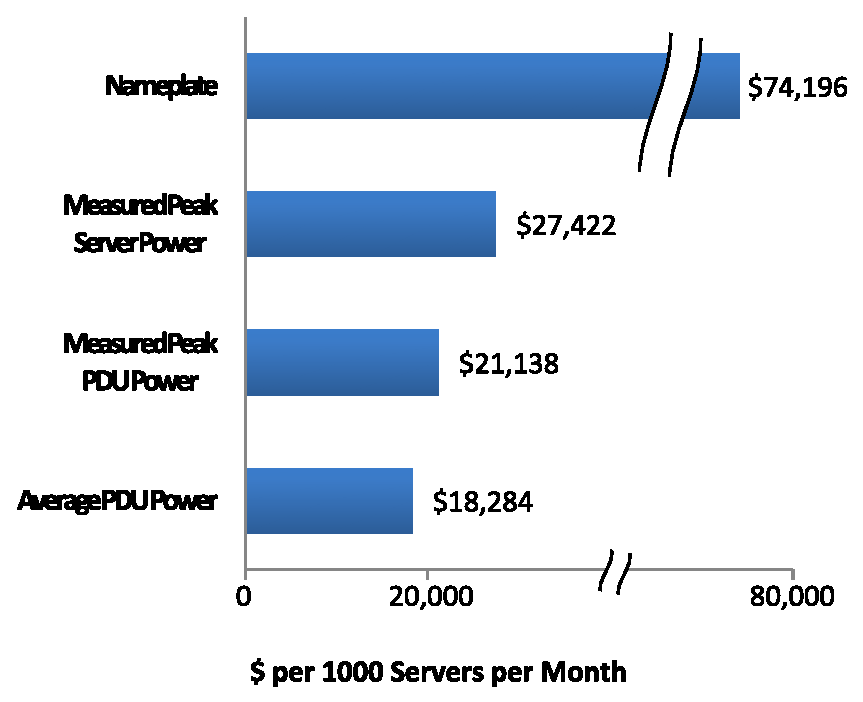
\includegraphics[width = 3.0 in]{Appendices/PowerRouting/figure/intro.eps}
\vspace{-.05 in}
\caption{ \textbf{The cost of over-provisioning.} \textnormal{Amortized monthly cost of power infrastructure for 1000 servers under varying provisioning schemes.}}
\label{figure::intro}
\vspace{-.1 in}
\end{figure}

Although the power demands of individual servers can vary greatly, statistical effects make it unlikely for all servers' demands to peak at the same time \cite{Govindan09,Ranganathan06}. Even in highly-tuned clusters running a single workload, peak utilization is rare, and still falls short of provisioned power capacity \cite{Fan07}.  This observation has lead researchers and operators to propose \emph{over-subscribing} power circuits.  To avoid overloads that might impact availability, such schemes rely on \emph{power capping} mechanisms that enforce power budgets at individual servers \cite{Lefurgy08, Wang08} or over ensembles \cite{Ranganathan06, Wang09}.  The most common power-capping approaches rely on throttling server performance to reduce power draw when budgets would otherwise be exceeded \cite{Lefurgy08,Ranganathan06, Wang08,Wang09}.  

Figure~\ref{figure::intro} illustrates the cost of conservative provisioning and the potential savings that can be gained by over-subscribing the power infrastructure.  The graph shows the amortized monthly capital cost for power infrastructure under varying provisioning schemes.  We calculate costs following the methodology of Hamilton \cite{Hamilton09} assuming high-availability power infrastructure costs \$15 per critical-load Watt \cite{Turner06}, the power infrastructure has a 15-year lifetime, and the cost of financing is 5\% per annum.   We derive the distribution of actual server power draws from 24 hours of data collected from 1000 servers in three production facilities (details in Section \ref{section::methodology}).  Provisioning power infrastructure based on nameplate ratings results in infrastructure costs over triple the facility's actual need.  Hence, operators typically ignore nameplate ratings, instead provisioning infrastructure based on a measured peak power for each class of server hardware.  However, even this provisioning method overestimates actual needs---provisioning based on the observed aggregate peak at any power distribution unit (PDU) reduces costs 23\%. Provisioning for less-than-peak loads can yield further savings at the cost of some performance degradation (e.g., average power demands are only 87\% of peak).  

Power capping makes over-subscribing safe.  However, power budgets must enforce local (PDU) as well as global (uninterruptible power supply, generator and utility feed) power constraints.  Hence, local spikes can lead to sustained performance throttling, even if the data center is lightly utilized and ample power delivery capacity is available elsewhere.  Moreover, in high-availability deployments, the need to maintain reserve capacity on redundant power delivery paths to ensure uninterrupted operation in the event of PDU failure magnifies the impact of utilization spikes---not only does the data center's direct demand rise, but also the potential load from failover.

An ideal power delivery system would balance loads across PDUs to ensure asymmetric demand does not arise.  Unfortunately, since server power demands vary, it is difficult or impossible to balance PDU loads statically, through clever assignment of servers to PDUs.  Such balancing may be achievable dynamically through admission control \cite{Chase01} or virtual machine migration \cite{Clark05}, but implies significant complexity, may hurt performance, and may not be applicable to non-virtualized systems. Instead, in this paper, we explore mechanisms to balance load through the \emph{power delivery infrastructure}, by dynamically connecting servers to PDUs. 

Our approach, \emph{Power Routing}, builds on widely-used techniques for fault-tolerant power delivery, whereby each server can draw power from either of two redundant feeds.  Rather than designating primary and secondary feeds and switching only on failure (or splitting loads evenly across both paths), we instead centrally control the switching of servers to feeds.  The soft-switching capability (already present  for ease of maintenance in many dual-corded power supplies and rack-level transfer switches) acts as the foundation of a power switching network.

In existing facilities, it is common practice for all servers in a rack or row to share the same pair of redundant power feeds, which makes it impossible to use soft-switching to influence local loading.  Our key insight, inspired by the notion of skewed-associative caches \cite{Seznec93} and declustering in disk arrays \cite{Alvarez98}), is to create \emph{shuffled distribution topologies}, where power feed connections are permuted among servers within and across racks. In particular, we seek topologies where servers running the same workload (which are most likely to spike together) connect to distinct pairs of feeds.  Such topologies have two implications.  First, they spread the responsibility to bear a failing PDU's load over a large number of neighbors, reducing the required reserve capacity at each PDU relative to conventional designs.  Second, they create the possibility, through a series of switching actions, to route slack in the power delivery system to a particular server.

Designing such topologies is challenging because similar servers tend to be collocated (e.g., because an organization manages ownership of data center space at the granularity of racks).  Shuffled topologies that route power from particular PDUs over myriad paths require wiring that differs markedly from current practice.  Moreover, assignments of servers to power feeds must not only meet PDU capacity constraints, they must also: (1) ensure that no overloads occur if any PDU fails (such a failure instantly causes all servers to switch to their alternate power feed); and (2) balance power draws across the three phases of each alternating current (AC) power source to avoid voltage and current fluctuations that increase heating, reduce equipment lifetime, and can precipitate failures \cite{Gruzs90}. Even given a shuffled topology, power routing remains challenging: we will show that solving the dynamic assignment of servers to PDUs reduces to the partitioning problem \cite{GareyBook}, and, hence, is NP-complete and infeasible to solve optimally.  In this paper, we address each of these challenges, to contribute:

\begin{packed_itemize}

\item {\bf Lower reserve capacity margins.}   Because more PDUs cooperate to tolerate failures, shuffled topologies reduce per-PDU capacity reserves from 50\% of instantaneous load to a $1/N$ fraction, where $N$ is the number of cooperating PDUs.   
\vspace{4pt}
\item {\bf Power routing.} We develop a linear programming-based heuristic algorithm that assigns each server a power feed and budget to minimize power capping, maintain redundancy against a single PDU fault, and balance power draw across phases.
\vspace{4pt}
\item {\bf Reduced capital expenses.}  Using traces from production systems, we demonstrate that our mechanisms reduce power infrastructure capital costs by 32\% without performance degradation.  With energy-proportional servers, savings reach 47\%.

\end{packed_itemize}

The rest of this paper is organized as follows.  In Section~\ref{section::background}, we provide background on data center power infrastructure and power capping mechanisms.   We describe our mechanisms in Section~\ref{section::powerrouting} and detail \PowerRouting's scheduling algorithm in Section~\ref{section::scheduling}.  We evaluate our techniques on our production data center traces in Section~\ref{section::evaluation}.  Finally, in Section~\ref{section::conclusion}, we conclude. 
